
\documentclass[11pt,a4paper]{article}
\usepackage[left=2cm,right=2cm,top=2cm,bottom=3cm]{geometry}
\usepackage{amsmath,amsfonts,amsthm,amssymb,varioref,times, commath}
\usepackage{gensymb}
\usepackage{tikz}
\usepackage{textcomp}
\usepackage{hyperref}
\hypersetup{
 colorlinks=true,
 linkcolor=blue,
 filecolor=magenta, 
urlcolor=cyan,
}
\usepackage{lipsum}
\usepackage{epigraph}
%to resume numbering in a list
\usepackage{enumitem}
%----- arrows 
\usepackage{extarrows}

%    differential equatiosn 
\usepackage{diffcoeff}   %\diff[2]{x}{y}


%%%%%%pour ecrire en français avec les accents
\usepackage[utf8]{inputenc}
\usepackage[T1]{fontenc}
\usepackage{lmodern} % load a font with all the characters
\usepackage{units}
%%%%%%%Image-related packages
\usepackage{wrapfig}
\usepackage{float, graphicx}
\graphicspath{ {./img/} }
\usepackage{subcaption}
\usepackage[export]{adjustbox}

%%%%%%%pour faire des cadres
\usepackage{xcolor}
\usepackage{tcolorbox}
\usepackage{framed}
\usepackage{mdframed}


%%%%%%%chemistry frmulae
\usepackage{chemfig}
\usepackage{chemformula}
\usepackage[version=4]{mhchem}

% -------------- Circuits -------------------
\usepackage[european, straightvoltages]{circuitikz}

% Title & headers
\usepackage[explicit]{titlesec}
% Raised Rule Command:
% Arg 1 (Optional) - How high to raise the rule
% Arg 2 - Thickness of the rule
\newcommand{\raisedrulefill}[2][0ex]{\leaders\hbox{\rule[#1]{1pt}{#2}}\hfill}
\titleformat{\section}{\Large\bfseries}{\thesection. }{0em}{#1\,\raisedrulefill[0.4ex]{1pt}}

% pour ecrire sur +sieurs colonnes
\usepackage{multicol}
\setlength{\columnseprule}{0pt}
\setlength{\columnsep}{60pt}
% Fusion de lignes de tableaux.
\usepackage{multirow}
% Position verticale des lettres dans la ligne de tableau.
\usepackage{array}

% physics -----------------------------------------------------------
\newcommand{\To}{\longrightarrow}
\newcommand{\gpl}{\; g\cdot L^{-1}}
\newcommand{\gpmol}{\; g\cdot mol^{-1}}
\newcommand{\mpl}{\; mol\cdot L^{-1}}
\newcommand{\mps}{\; m\cdot s^{-1}}
\newcommand{\rps}{\; rad\cdot s^{-1}}
\newcommand{\kph}{\; km\cdot h^{-1}}
\newcommand{\mpss}{\; m\cdot s^{-2}}
\newcommand{\Dt}{\Delta t}
\newcommand{\vv}{\vec{v}}
\newcommand{\va}{\vec{a}}
\newcommand{\vp}{\vec{p}}
\newcommand{\vf}{\vec{F}}
\newcommand*{\Vf}[1]{\overrightarrow{F_\ensuremath{{#1}}}}
\newcommand{\es}[1]{\cdot10^{#1}}
\newcommand{\eng}[1]{\textcolor{purple}{(= #1})}
\usepackage{harpoon}
%\newcommand*{\vect}[1]{\overrightharp{\ensuremath{#1}}}
\newcommand*{\Vect}[1]{\overrightarrow{\ensuremath{#1}}}
\newcommand{\pfd}[1]{\sum \vec{F}_{ext_{#1}} &= \od{\vp_{#1}}{t} = m\cdot\va_{#1}}
\newcommand{\C}{\degree C}
\newcommand{\Delt}{\Delta t}

% --- Circuits ------------
\newcommand{\bipole}[1]{
\begin{circuitikz} \draw
(0,0) to[ #1 ] (2,0); 
\end{circuitikz} {\hspace{5mm}}}

% Chimie ---------------------------------
\newcommand{\oxo}{\ce{H3O+}_{(aq)}}
\newcommand{\eau}{\ce{H2O}_{(\ell)}}
\newcommand{\OH}{\ce{HO-}_{(aq)}}
\newcommand{\AH}{\ce{AH}_{(aq)}}
\newcommand{\A}{\ce{A-}_{(aq)}}
\newcommand{\MnO}{\ce{MnO_4^{-}}}
\newcommand{\conc}[1]{\left[{#1}\right]}
\newcommand{\couple}[2]{\ce{#1/#2}}


% Environnements ------------------------
\newcounter{exo}
\newenvironment{exo}[1][]
{\refstepcounter{exo} \begin{shaded}\noindent $\triangleright \quad$\textbf{Exercice~\theexo. #1} } { \end{shaded}}
\newenvironment{eg}
{\begin{shaded} \textbf{Exemple:} } { \end{shaded}}

\newenvironment{defn}[1]
{\begin{leftbar}\noindent \textbf{Définition :\textit{ \quad #1}} } { \end{leftbar}}

%\newenvironment{rmrq}
%{\begin{shaded} \textbf{Remarque.\quad } \itshape } { \end{shaded}}
\newenvironment{rmrq}
{\begin{mdframed}[backgroundcolor=blue!10, linewidth=0pt] \textbf{Remarque.\quad } \itshape } { \end{mdframed}}

\newenvironment{python}
{\begin{shaded} \textbf{A faire en PYTHON}\\ \itshape } { \end{shaded}}

% Shading colour -----------------------------
\definecolor{shadecolor}{gray}{0.9}

\date{}
\author{}

\renewcommand*\contentsname{Résumé}









% Title & headers 
\usepackage{fancyhdr}
\pagestyle{fancy}
\fancyhf{}
\lhead{SciPhy : Terminale spé}
\rhead{$\Phi $ - 7 : Circuits}
\chead{2020-28}
\rfoot{Page \thepage}
\lfoot{\textcopyright\; S Zayyani}
\renewcommand{\footrulewidth}{0.1pt}% default is 0pt

\title{\large Physique - Chapitre 7 \\ \LARGE  Les circuits électroniques}
\date{}
\author{}

\setlength{\parindent}{0mm}
\setlength{\parskip}{2mm}

%%%%%%%%%%% For wrapfigure 
\setlength{\intextsep}{5pt}%
\setlength{\columnsep}{7pt}%



\begin{document}
\maketitle
\vspace{-1cm}
\begin{tcolorbox}[title=Notions de la classe de première à rappeler]
calcul d'un logarithme ; solvatation d'un proton libre dans l'eau ; Concentration molaire
%\tcblower
\end{tcolorbox}
\tableofcontents

%%%%%%%%%%%%%%%%%%%%%%%%%%%%%%% Section 1 %%%%%%%%%%%%%%%%%%%%%%%%%%%%%
\section{Rappels (du collège \& de la seconde)}
Nous allons commencer par quelques rappels des notions sur les circuits électriques que vous auriez du voir au collège. Il s'agit principalement de  définitions.

\subsection{Dipôles électriques}

Les dispositifs que l'on voit au collège et au lycée sont presque exclusivement des dipôles. 

\begin{table}[ht]
    \centering
    \begin{tabular}{|| c  c | c  c | c  c ||}
     \hline\hline 
     Pile  &  \begin{circuitikz}[european] \draw (0,0) to[battery1] (2,0); \end{circuitikz} &  Générateur  &  \begin{circuitikz}[european] \draw (0,0) to[vsource] (2,0); \end{circuitikz}  &   Interrupter &  \begin{circuitikz}[european] \draw (0,0) to[normal open switch] (2,0); \end{circuitikz} \\[2.5ex]
     \hline
     Voltmètre      &  \begin{circuitikz}[european] \draw (0,0) -- (0.5,0) ; \filldraw [fill=white,draw=black] (1,0) circle (0.5cm) node {V};\draw (1.5,0) -- (2,0); \end{circuitikz} & Résistance      &  \begin{circuitikz}[european] \draw (0,0) to[generic] (2,0); \end{circuitikz} & Lampe      &  \begin{circuitikz}[european] \draw (0,0) to[lamp] (2,0); \end{circuitikz} \\[2.5ex]
     \hline 
     Ampèremètre &  \begin{circuitikz}[european] \draw (0,-1) -- (0.5,-1) ; \filldraw [fill=white,draw=black] (1,-1) circle (0.5cm) node {A};\draw (1.5,-1) -- (2,-1); \end{circuitikz} &  Diode      &  \begin{circuitikz}[european] \draw (0,0) to[diode] (2,0); \end{circuitikz} &  DEL      &  \begin{circuitikz}[european] \draw (0,0) to[led] (2,0); \end{circuitikz} 
     \\[2.5ex]
     \hline
     Condensateur      &  \begin{circuitikz}[european] \draw (0,0) to[capacitor] (2,0); \end{circuitikz} & Bobine (inducteur)      &  \begin{circuitikz}[european] \draw (0,0) to[cute inductor] (2,0); \end{circuitikz} &  Moteur      &  \begin{circuitikz}[european] \draw (0,0) -- (0.5,0) ; \filldraw [fill=white,draw=black] (1,0) circle (0.5cm) node {M};\draw (1.5,0) -- (2,0); \end{circuitikz} \\[2.5ex]
     \hline\hline
\end{tabular}
    \caption{Un tableau récapitulatif des dipôles les plus fréquemment utilisés.}
\end{table}
%\vspace{1cm}
\begin{defn}{Dipôle électrique}
\begin{itemize}
    \item Un \textbf{dipôle} est un composant électrique avec une entrée de courant et une sortie, d'où l'appellation \textit{di}pôle. 
    \item Les dipôles tombent en deux catégories : générateur ou récepteur\eng{electrical load}
    \begin{itemize}
        \item \textbf{Générateur} : Un dipôle qui \textbf{fournit l'énergie électrique} au circuit. Il le fait en convertissant une forme d'énergie en énergie électrique (générant ainsi une tension électrique entre ses bornes), et ce qui permet le courant électrique de circuler dans le circuit. 
        \item \textbf{Récepteur} : Un dipôle qui effectue un 'action' grâce au courant électrique qui le traverse. Autrement dit, qui \textbf{convertit l'énergie électrique du circuit en une autre forme d'énergie}. 
    \end{itemize}
\end{itemize}
\end{defn}

\subsection{Intensité du courant \& Tension électrique}

\begin{multicols}{2}
\begin{defn}{Tension électrique}
\begin{itemize}
    \item La tension électrique $U$ , est la \textbf{différence de potentiel électrique} $V_A$ et $V_B$ entre deux points différents (du circuit) : 
    \[ U_{AB} = V_B - V_A \]
    \item La tension s'exprime en $Volts\; V$. 
    \item La tension électrique entre deux points d'un circuit se mesure grâce à un \textit{voltmètre}. 
    \item Un voltmètre est branché \textbf{en dérivation} par rapport aux deux points. Si branché en série, il se comporte comme un interrupteur ouvert. 
\end{itemize}
\end{defn}
\begin{defn}{Intensité du courant}
\begin{itemize}
    \item L'intensité du courant, noté $I$ ou $i$, est une mesure de la \textbf{quantité de charge électrique (notée $Q$ ou $q$) qui passe devant un point du circuit en une seconde} : $I = \nicefrac{Q}{\Delta t}$
    \item Le débit/intensité instantané est donné par : \[i(t) = \od{q}{t}\]
    \item L'intensité du courant s'exprime en \emph{ampère} $A=C\cdot s^{-1}$. 
    \item L'intensité se mesure grâce à un \textit{ampèremètre}\eng{ammeter}. 
    \item Un ampèremètre est branché \textbf{en série} dans un circuit. Si branché en dérivation, cela fera un court-circuit. 
\end{itemize}
\end{defn}
\end{multicols}

\begingroup
\begin{wrapfigure}{r}{0.4\textwidth}
    \centering
    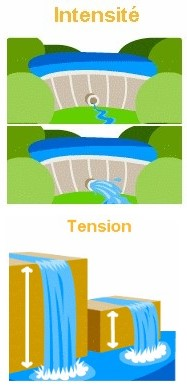
\includegraphics[width=0.85\linewidth]{imgs/p7/analogie.jpg}
\end{wrapfigure}
\begin{rmrq}
Tandis que l'intensité du courant est une notion facile à comprendre et à visualiser, la notion de tension électrique est plus difficile à saisir, à première vue. D'une part, une analogie simple qui permet de mieux voir l'intensité du courant serait de compter le nombre de personnes qui passent devant un point pendant une période: plus il y a de personnes qui passe, plus le \textit{courant} est intense (ici les \textit{personnes} sont l'équivalent des électrons, par exemple, ou plus généralement de la charge électrique). 

D'autre part la tension électrique est aux différence de potentiels gravitationnels. Si nous mettons un ballons sur une terre plate, il ne bougerait pas. Si on le met sur une légère pente, il commence à rouler doucement vers le bas. Ceci est du à la différence de potentiel gravitationnel, car la position de départ et de la fin ne sont pas à la même hauteur, autrement dit aux différents potentiels gravitationnels. Plus cette différence est importante, plus le ballon roule avec une vitesse importante, et plus il peut surmonter, par exemple, les obstacles sur son chemin. La situation est quasi-identique avec une particule chargée dans un champ électrique. La tension générée par un pile par exemple est la différence de potentiel électrique entre sa sortie et son entrée. C'est cette différence qui donne l'impulsion aux particules chargées pour se déplacer dans le circuit.  
\end{rmrq}

\endgroup

\subsection{Circuit électrique}
Un circuit électrique est un ensemble de conducteurs et de dispositifs électriques, reliés entre eux par des fils électriques. Un circuit comporte, presque toujours, un ou plusieurs générateur qui est la source de l'énergie électrique qui circule dans le circuits, et d'un ou plusieurs récepteur qui reçoivent cette énergie électrique afin de le convertir en une autre forme d'énergie (mécanique, ou thermique par exemple. 

\subsubsection*{Le sens du courant}

Un courant électrique est la manifestation des charges électriques qui se déplace. Dans un solide ces charges sont des électrons qui se déplacent dans le matériau conducteur (dans ce qu'on appelle la bande de conduction). Mais dans un liquide (ou solution) ce sont des particules chargées, autres qu'électrons, qui sont responsable pour le courant électrique, des ions par exemple.

Les caractéristiques du courant, son sens et son intensité sont imposés par le générateur. \textbf{A l'extérieure d'un générateur, le courant électrique va de la borne $+$ vers la borne $-$ du générateur}. 

\begin{center}
    \begin{circuitikz}
    \draw (0,0) to[battery1,*-*, v<=$U$, i<=$ $] (3,0) ; 
    \draw (0.9,0.3) node{$+$};
    \draw (2.1,0.3) node{$-$};    
    \end{circuitikz}
    \hspace{3cm}
    \begin{circuitikz}
    \draw (0,0) to[vsource,*-*, v<=$U$, i<=$ $] (3,0) ; 
    \draw (0.9,0.3) node{$+$};
    \draw (2.1,0.3) node{$-$};    
    \end{circuitikz}   
\end{center}

\begin{rmrq}
Nous savons que le courant est dû au mouvement des électrons dans les fils. Or les électrons, négativement chargés, vont vers le pôle $+$ du générateur. Cela veut dire que le sens de circulation des électrons est de $-$ vers $+$, c'est à dire le sens opposé au mouvement! 

La raison est plutôt historique : l'étude de l'électricité et de ses propriétés date du $XVIII^e$ siècle, alors que l'électron n'a été découvert qu'en 1897 (par J.J.Thompson). Toute la description des courants électriques été basée donc sur l'idée que les porteurs de charges étaient positivement chargés. Ce qu'on appelle aujourd'hui des \emph{trous}. 
\end{rmrq}

\subsubsection*{Branchement en série \& en dérivation}

\begin{figure}[h]
    \centering
\begin{circuitikz}
\draw (0,4) to[short, i=$i$] (2,4) to [R, i=$i_1$, l=$R_1$] (2,0) ;
\draw (2,4) -- (4,4) to[R, l=$R_2$, i=$i_2$] (4,0) -- (0,0) ;
\filldraw[black] (2,4) circle (1pt) ;
\filldraw[black] (2,0) circle (1pt) ;
\filldraw[black] (0,4) circle (1pt) ;
\filldraw[black] (0,0) circle (1pt) ;
%\draw [->, thick] (0,0.2) -- (0,3.8) ; 
%\draw (0,2) node [anchor=west] {$U$}; 
\end{circuitikz}
\hspace{3cm}
\begin{circuitikz}
\draw (0,4) to[short, i=$i$] (2,4) to[R, i=$ $, l=$R_1$] (2,2) to[R, l=$R_2$]  (2,0) to[short, i=$ $] (0,0) ;
\filldraw[black] (0,4) circle (1pt) ;
\filldraw[black] (0,0) circle (1pt) ;
\end{circuitikz}
    \caption{Branchement en dérivation à gauche, en série à droite}
\end{figure}


\subsubsection*{Conventions récepteur \& générateur}

Comme nous l'avons déjà mentionné, un générateur fournit l'énergie électrique au circuit, tandis que les récepteur la consomme, ou convertissent en une autre forme. Ceci se manifeste en une variation du potentiel électrique opposée entre les récepteurs et les générateurs. Autrement dit un générateur augment la différence de potentiel électrique, et un récepteur diminue le potentiel électrique. La tension entre les bornes d'une générateur n'a pas le même signe que la tension entre les bornes d'un récepteur, comme on va voir. 

\begingroup
\begin{wrapfigure}{r}{0.4\textwidth}
\centering
        \begin{circuitikz}
        \draw (0,0) to[lamp,*-*, i<=$ $, v^=$U_R$] (3,0) ; 
        \end{circuitikz}  
        \caption{Convention générateur.}
        \vspace{0.35cm}
        \begin{circuitikz}
        \draw (0,0) to[battery1,*-*, v<=$U$, i<=$ $] (3,0) ; 
        \draw (0.9,0.3) node{$+$};
        \draw (2.1,0.3) node{$-$};    
        \end{circuitikz} 
        \caption{Convention récepteur.}
\end{wrapfigure}

Dans représentation symbolique des diagrammes de circuit, ceci est est traduit par le sens de la flèche indiquant la tension du dipôle. Nous parlons alors de la convention générateur, et convention récepteur. 

\begin{itemize}
    \item \textbf{Convention générateur} : le sens de la flèche de la tension est le même que celui du courant.
    \item \textbf{Convention récepteur} : le sens de la flèche de la tension est opposé au celui du courant. 
\end{itemize}

\endgroup
\newpage

\begin{eg}
\begingroup
\begin{wrapfigure}{r}{0.35\textwidth}
\begin{center}
    \begin{circuitikz}
        \draw (0,3) to[battery1, i=$i$] (0,0); 
        \draw (0,3) -- (3,3) to[lamp, i=$i$](3,0) -- (0,0); 
        \draw [fill] (1.5,3) circle [radius=0.05]; 
        \draw [fill] (1.5,0) circle [radius=0.05];  
        \draw [->, thick] (1.5,0.2) -- (1.5,2.8);
        \node [left] at (1.5,1.5) {$U$}; 
    \end{circuitikz}
\end{center}
\end{wrapfigure}
Considérons le circuit très simple ci-contre. Il s'agit d'un générateur et un récepteur, ici une lampe. 

La tension entre deux points d'un circuit est toujours la même $U$. On voit donc que du point de vu du générateur cette tension est dans le même sens que le courant, tandis que pour le récepteur cette tension va au sens opposé au courant. Voici donc les conventions générateur et récepteur. \vspace{1cm}

\endgroup
\end{eg}

%%%%%%%%%%%%%%%%%%%%%%%%%%%%%%% Section 2 %%%%%%%%%%%%%%%%%%%%%%%%%%%%%
\subsection{Les Lois de Kirchoff}
Nous avons vu au collège qu'il existe principalement deux types de circuits : \textbf{en série} (avec une seule boucle, ou \textbf{une seule maille}), et \textbf{en dérivation} (avec \textbf{plusieurs boucles ou mailles}). 

Les lois qui nous disent comment la tension et l'intensité du courant se comportent dans des différents types de circuits, s'appellent les lois de Kirchoff \eng{Kirchoff's circuit laws}, d'après l'allemand Gustav Kirchoff : 
\begin{itemize}
    \item \textbf{$1^{ère}$ loi de Kirchoff} : Loi des mailles, concernant la division de la tension dans une maille. 
    \item \textbf{$2^{ème}$ loi de Kirchoff} : Loi des noeuds, concernant la division du courant dans un noeud. 
\end{itemize}

\subsection*{Loi des Mailles}
\begin{shaded}
\textbf{Dans chaque maille d'un circuit, la somme algébrique des tensions de tous les dipôles de la maille est toujours zéro.}
\end{shaded}

\begingroup
\begin{wrapfigure}{r}{0.4\textwidth}
\begin{center}
    \begin{circuitikz}
        \draw (0,4) to[V, v<=$U_G$, i<=$i$] (0,0)  ; 
        \draw (0,4) --(1,4)  to [R, l^=$R_1$, v<=$U_1$, i=$i$] (3,4) -- (4,4) -- (4,3) to[R, l^=$R_2$, v<=$U_2$](4,1) -- (4,0) -- (3,0) to [R, l^=$R_3$, v<=$U_3$] (1,0) -- (0,0); 
        \vspace{1cm}
    \end{circuitikz}
\end{center} 
\caption{Une maille d'un circuit.}
\end{wrapfigure}

Dans le circuit ci-contre, d'après la loi des mailles on doit avoir la somme de toutes les tensions égale à $0$. Mais d'après la convention générateur, comme nous voyons sur le schéma le sens de la tension $U_G$ est opposé aux autres tension, et donc on en arrive à la relation : 
\begin{align*}
    0 &=-U_G + U_1 + U_2 + U_3  \\
    U_G &= U_1 + U_2 + U_3
\end{align*}

Si l'on voulait interpréter le sens de cette relation, ou de la loi des mailles, on peut tout simplement dire que la tension générée par le générateur est égale à la somme des tension utilisée par les récepteur. Autrement, l'énergie consommée par l'ensemble des récepteurs est égale à l'énergie fournie par l'ensemble des générateurs. 

\endgroup

\subsection*{Loi des Noeuds}
\begin{shaded}
\textbf{Dans chaque noeud d'un circuit électrique, la somme algébriques des intensités du courant entrant et sortant du noeud, est toujours nulle.}
\end{shaded}

\begingroup
\begin{wrapfigure}{r}{0.2\textwidth}
    \centering
    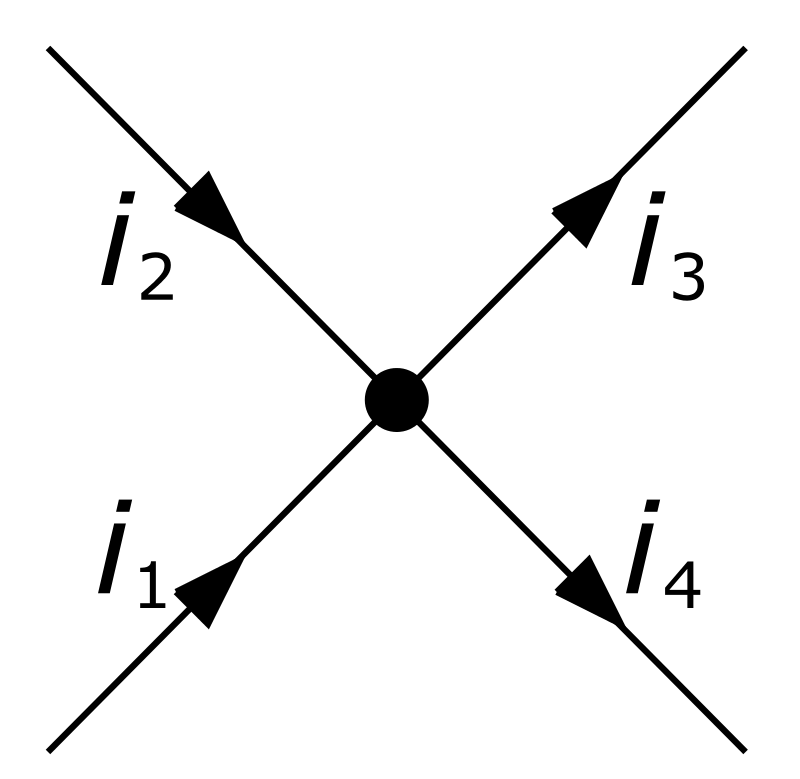
\includegraphics[width=0.9\linewidth]{imgs/p7/noeud.png}
    \caption{Un noeud dans un circuit.}
\end{wrapfigure}

Dans la figure ci-contre on voit un noeud quelconque dans un circuit. On voit clairement qu'il y a deux courant qui entrent dans le noeud, et deux qui sortent. D'après la loi des noeuds donc, la somme de ces quatre intensités doit être nulle. 

Mais il faut respecter le signe algébrique de chaque courant, c'est à dire quand le courant entre $i>0$, et quand le courant sort $i<0$. La relation mathématique relevant de la loi des noeuds est donc : 
\begin{align*}
    i_1 + i_2 - i_3 - i_4 &= 0 \\
    i_1 + i_2 &= i_3 - i_4
\end{align*}

\endgroup
Ce résultats, et la loi des noeuds, est plutôt facile à interpréter. L'intensité du courant est une mesure du débit de charge électrique. Dans ce cas-là dit simplement qu'autant de charge sort d'un noeud, qui y entre, et l'inverse. 


\begin{rmrq}
Les deux lois de Kirchoff sont les manifestations de deux principes fondamentaux et importants de la physique. La loi des mailles est une conséquence du principe de la \textbf{conservation de l'énergie}, et la loi des noeuds est une conséquence du principe de la \textbf{conservation de la charge électrique}. 
\end{rmrq}

%%%%%%%%%%%%%%%%%%%%%%%%%%%%%%% Section 3 %%%%%%%%%%%%%%%%%%%%%%%%%%%%%
\subsection{Le conducteur ohmique}

Une des manières la plus courante d'étudier le comportement d'un dipôle électrique, est grâce à sa \textbf{courbe caractéristique} \eng{current-voltage characteristic} (parfois appelé simplement sa \textit{caractéristique}). 

Il s'agit d'un graphique qui montre l'évolution de la tension $U$ entre les bornes du dipôle en fonction de $I$, l'intensité du courant qui le parcourt (i.e. le graphique $U=f(I)$). Dans certains livre la caractéristique peut être donnée comme $I=f(U)$. Cela n'est qu'un changement de représentation, et ne change pas le fond de ce que la caractéristique révèle. 


\subsubsection*{Conducteur Ohmique}

\begingroup
\setlength{\intextsep}{1pt}%
\begin{wrapfigure}{r}{0.25\textwidth}
\centering
    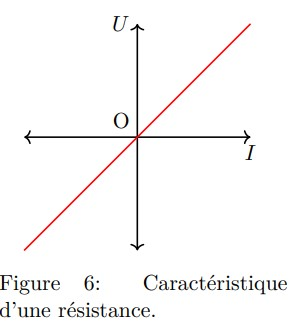
\includegraphics[width=0.95\linewidth]{imgs/p7/car1.jpg}
\end{wrapfigure}

Vous connaissez déjà le conducteur ohmique depuis la classe de quatrième. C'est le dipôle récepteur le plus simple que vous avez rencontré, avec le symbole\bipole{R}. 

Le conducteur ohmique est la catégorie des dipôles ayant un comportement caractérisé par la courbe caractéristique ci-contre. Autrement dit, tous dipôles ayant une tension qui varie de manière linéaire en fonction de l'intensité du courant. 

\endgroup

\subsubsection*{La loi d'Ohm}
La variation de $U$ en foncions de $I$ étant linéaire, on peut le modéliser mathématiquement par une fonction du type $y = m\cdot x$, où $m$ est le coefficient directeur du graphique précédent, c'est à dire la constante de proportionnalité entre la tension $U$ et l'intensité $I$. Dans notre modélisation donc l'ordonnée $y$ correspond à la tension $U$, et l'abscisse $x$ correspond à l'intensité $I$, ce qui donne une loi que vous connaissez déjà : La loi d'Ohm.

Avec $R$ comme constante de proportionnalité. 

\begin{defn}{Loi d'Ohm}
\begin{itemize}
    \item La loi d'Ohm est une loi empirique liant l'intensité du courant traversant un conducteur ohmique, et la tension entre ses bornes. 
    \item Elle s'exprime mathématiquement : 
    \[ U = R\cdot I \]
    \item La constante de proportionnalité $R$ s'appelle la résistance du conducteur ohmique, et est une mesure, justement, de la résistance à l'intérieur du conducteur, au passage du courant électrique. 
    \item $R$ s'exprime en \emph{ohm}, noté par le symbole $\ohm$ (omega majuscule). 
\end{itemize}
\end{defn}



\subsubsection*{Le générateur}
\begingroup

\begin{wrapfigure}{l}{0.5\textwidth}
\centering
    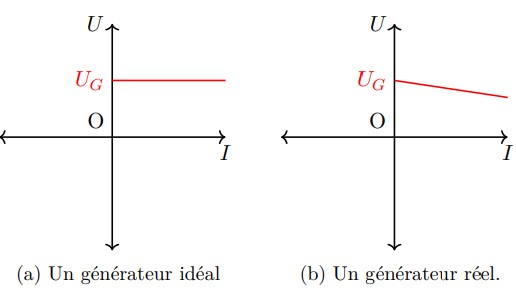
\includegraphics[width=0.95\linewidth]{imgs/p7/car2.jpg}
\end{wrapfigure}
Nous n'allons pas entrer trop en détails cette année des différents types de générateur que l'on peut avoir (e.g. générateur de tension idéal, générateur de courant idéal, etc.), mais l'essentiel ne change pas : un générateur doit fournir l'énergie électrique au circuit, et est caractérisé par une tension qui doit rester plus ou moins constante et stable. 


Nous faisons la distinction entre un générateur \textbf{idéal} et un générateur \textbf{réel}. C'est d'ailleurs une distinction que nous faisons souvent. La \textbf{différence entre un dipôle réel et idéal est la présence d'une petite résistance interne}. Un dipôle idéal, est tel, car on suppose qu'il n'y a aucune résistance au passage du courant à son intérieur, tandis que dans le monde réel, tout dipôle possède une certaine résistance interne, même si elle peut être très faible. 

\endgroup
Un générateur idéal arrive à maintenir la tension qu'il génère, alors qu'un générateur réel, perd une partie de l'énergie qu'elle produise en raison de cette résistance interne. La tension générée par un générateur réel, selon la courbe caractéristique ci-contre est de forme : 

\[ U = U_G - r\cdot I \quad \quad
\begin{cases}
r \text{ est la résistance interne du générateur}\\
U \text{ est la tension réelle fournie par le générateur}\\
U_G \text{ est la tension idéale (nominale) du générateur}\\
I \text{ est l'intensité du courant qui parcourt le générateur}
\end{cases}
\] 
 
\subsubsection*{Le point de fonctionnement}

Nous pouvons maintenant utiliser toutes les informations précédente afin de déterminer dans quel étant fonctionnerait notre circuit. Étant donné que dans un circuit simple (caractérisé par les courbes ci-contre), il faut la même tension électrique et intensité du courant dans le générateur que dans le dipôle ohmique y branché, le circuit fonctionnerait à l'intersection des deux caractéristiques. Ce point est nommé le \textbf{point de fonctionnement}. L'intensité du fonctionnement $I_f$ est donc l'intensité du courant qui circulerait dans le circuit, et la tension du fonctionnement $U_f$ serait la tensions entre les bornes du générateur et du récepteur. 

\begin{figure}[h]
\centering
    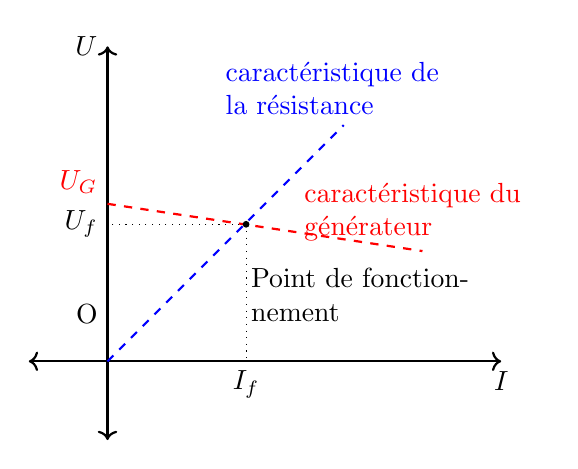
\begin{tikzpicture}[scale=2]
        \draw [thick] [<->] (0,-0.5) -- (0,2) node [left] {$U$};
        \draw (0,0.3) node [left] {O};
        \draw [thick] [<->] (-0.5,0) --++(3,0) node [below] {$I$};
        \draw [thick, red, dashed] [-] (0,1) node [anchor=south east]{$U_G$} --++ (2,-0.3) node[anchor=south, text width=3cm]{caractéristique du générateur} ; 
        \draw [thick, blue, dashed] [-] (0,0)  --++ (1.5,1.5) node[anchor=south, text width=3cm]{caractéristique de la résistance} ; 
        \filldraw[black] (0.88,0.87) circle (0.5pt) ;
        \draw (0.85,0.65) node[anchor=north west, text width=3cm] {Point de fonctionnement};
        \draw [dotted] (0.88,0.87) -- (0.88,0) node[anchor=north]{$I_f$} ; 
        \draw [dotted] (0.88,0.87) -- (0,0.87) node[anchor=east]{$U_f$} ;
        \end{tikzpicture}
\caption{Détermination graphique du point de fonctionnement.}
\end{figure}

Cette analyse est parfaitement valable pour des circuits encore plus compliqué, comportant par exemple plusieurs conducteurs ohmiques. 

\section{Le dipôle Condensateur}
En électronique il y a trois dipôles principaux que l'on étudie : la résistance (conducteur ohmique), le condensateur, et la bobine d'induction (inducteur). Il y a, bien sur, d'autres dipôles aussi, mais ces trois-là ont un comportement particulier chacun qui nous permet d'analyser de manière complète le comportement des circuits électroniques. 

\subsection{Principe de fonctionnement}

\begin{defn}{Condensateur\eng{capacitor}}
\begin{itemize}
    \item Un condensateur est un dipôle électronique composé de deux surface conductrices, appelées des armatures, séparées d'une distance. 
    \item Les armatures sont souvent plates et parallèles, séparées d'un isolant, souvent l'air. 
    \item Le symbole universel du condensateur est \bipole{C}. 
    \item Le condensateur est caractérisé par sa capacité $C$, qui s'exprime en $Farads\; (F)$. 
\end{itemize}
\end{defn}

Lorsqu'on applique une tension aux borne du condensateur, il y a une accumulation de charge $Q$ qui commence sur les armatures. Ceci est du à la présence de l'isolant entre ces deux dernières. Bien sur la capacité d'un condensateur dépend de divers facteurs : la surface des armatures, leur matériau, la distance entre elles, la nature de l'isolant, etc. \textbf{On peut considérer le condensateur donc comme un dipôle stockeur de charge. }

Le fonctionnement, et le comportement d'un condensateur est en raison de l'accumulation de la charge sur ses armatures (phase de charge), et la décharge de ses armatures (phase de décharge), où il perds la charge accumulée. La charge accumulée est créé une tension entre les bornes du condensateur, contre la tension imposée par le générateur. 

\subsection{Caractéristiques du condensateur}

La tension $u_C$ du générateur est donc proportionnelle à la charge accumulée $q$, et la capacité $C$ du condensateur: 
\begin{equation}
    u_C = \dfrac{q}{C} \quad \Longleftrightarrow \quad q=C\cdot u_C
\end{equation} 
 
La charge sur chaque armature est donc : $q^+ = C\cdot u_C$ et $q^- = -C\cdot u_C$. 

\begin{figure}[H]
\centering
\begin{subfigure}{.4\textwidth}
  \centering
  % include first image
  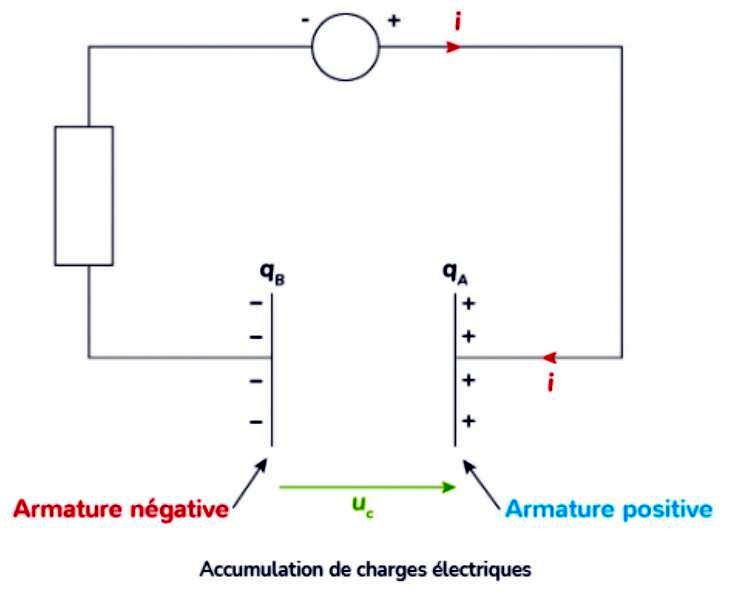
\includegraphics[width=.95\linewidth]{imgs/p7/condensateur.jpg}  
\end{subfigure}
\begin{subfigure}{.57\textwidth}
\begin{center}
    \begin{circuitikz}
        \draw (0,3) to[V, i=$i$] (0,0); 
        \draw (0,3) -- (3,3) to[C, i=$i$](3,0) -- (0,0); 
        \draw [fill] (1.5,3) circle [radius=0.05]; 
        \draw [fill] (1.5,0) circle [radius=0.05];  
        \draw [->, thick] (1.5,0.2) -- (1.5,2.8);
        \node [left] at (1.5,1.5) {$U_C$}; 
    \end{circuitikz}
\end{center}
\end{subfigure}
\caption{}
\end{figure}

Nous avons aussi maintenant tout ce qu'il nous faut pour établir une relation entre l'intensité (instantanée) du courant et la tension entre les bornes du condensateur : 

\begin{align}
    i &= \od{q}{t} = \od{\left(C\cdot u_C\right)}{t} \\
    i &=C\od{u_C}{t}
\end{align}

\section{Le circuit RC}

Un circuit contenant un conducteur ohmique $R$ et un condensateur $C$ s'appelle un circuit RC (quelle originalité, je sais). Ces dipôles peuvent être branchés en série ou en dérivation. Pour commencer nous nous intéressons aux cas les plus simples : le circuit RC en série. 

\subsection{Régime transitoire \& régime permanent}
La conducteur ohmique est un dipôle qui réagit de manière instantanée et proportionnelle à l'intensité du courant qui le parcourt. Avec l'inclusion du condensateur la réponse du système est plus ``lent'' dans ses réactions, c'est à dire qu'il faut un temps pour les tensions et les intensités se stabilisent. 

On fait donc la différence entre le \textbf{régime permanent} (ou continu, ou stationnaire) où les tensions et les intensité dans les branches du circuits et dans les dipôles se sont stabilisées, le \textbf{régime variable ou transitoire}  où les tensions et les intensité dans le circuit sont en cours de variation afin d'atteindre leurs valeurs stables en régime permanent. 

\begin{figure}[H]
    \centering
    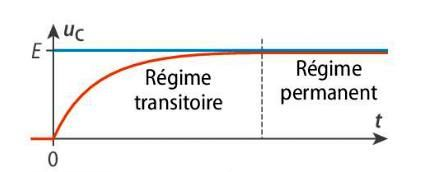
\includegraphics[width=0.8\linewidth]{imgs/p7/regimes.jpg}
\end{figure}

Considérons le circuit électrique ci-après (cf Figure.\ref{fig:decharge}). Nous allons donc étudier le comportement d'un condensateur en deux états : l'état de \textbf{charge}, et l'état de \textbf{décharge}. 

\begin{figure}[H]
\centering
\begin{subfigure}{.47\textwidth}
  \centering
  % include first image
  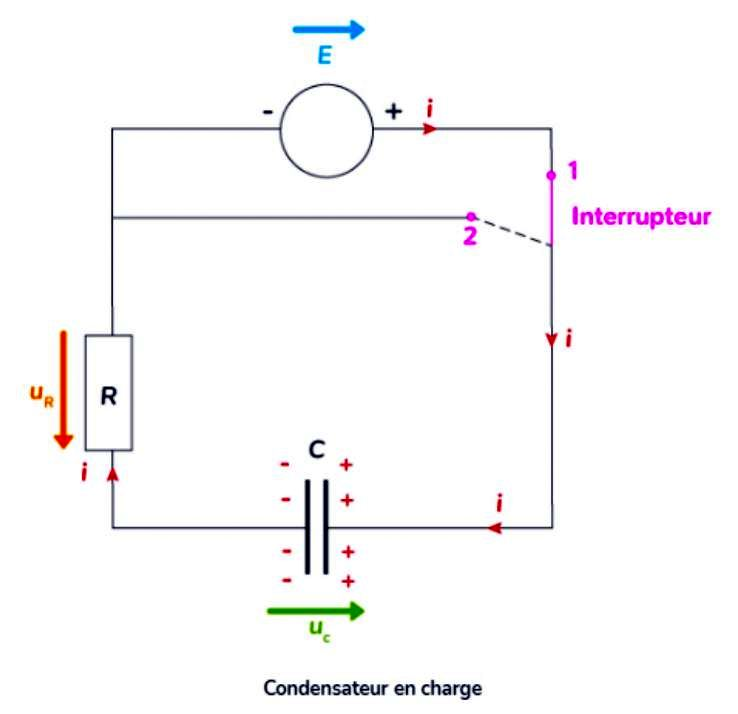
\includegraphics[width=\linewidth]{imgs/p7/RCcharge.jpg}  
\end{subfigure}
\begin{subfigure}{.47\textwidth}
  \centering
  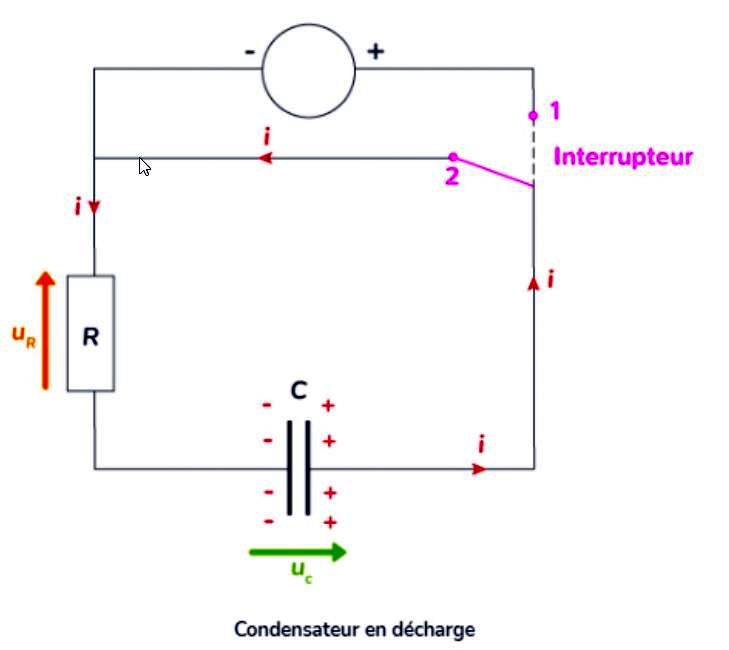
\includegraphics[width=.93\linewidth]{imgs/p7/RCdecharge.jpg}  
\end{subfigure}
\caption{Un circuit RC en deux modes : charge \& décharge}
\label{fig:decharge}
\end{figure}

Notre objectif principal dans les deux cas est d'obtenir l'équation (différentielle) du circuit, dont la solution nous permettant de modéliser l'évolution de la tension (ou de la charge électrique) dans le circuit. 

\subsection{Circuit de charge}

\begingroup
\setlength{\intextsep}{-15pt}%
\begin{wrapfigure}{r}{0.38\textwidth}
  \centering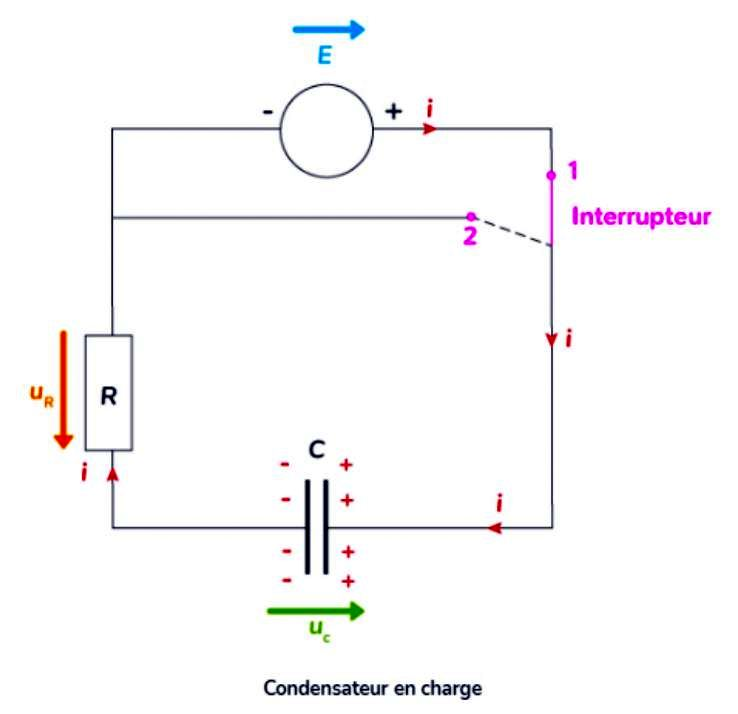
\includegraphics[width=\linewidth]{imgs/p7/RCcharge.jpg}
\end{wrapfigure}

Le circuit RC est en charge (ou simplement le condensateur est en charge) lorsqu'il est branché sur le générateur. Dans ce cas de figure le \textbf{condensateur est un récepteur} (convention récepteur donc à respecter pour les tensions et les courants). 

Afin d'obtenir l'équation différentielle du circuit \textbf{nous appliquons simplement la loi des mailles} à toutes les mailles concernées. Nous allons trouver l'équation différentielle du circuit en termes de $u_C$, mais aussi en termes de $q$, car les deux sont liées. 

\endgroup
\vspace{.5cm}
D'après la loi des mailles : 


\begin{align*}
    E - u_C - u_R &= 0 \\
    u_C + u_R &= E \\
    u_C + Ri &= E
\end{align*}
\begin{multicols}{2}
Pour trouver l'équation du système en termes de $u_C$ substituons avec $(3)$ : 
\[ u_C + RC\od{u_C}{t} = E\]

Mettons cette équation en forme canonique : 
\begin{equation}
    \od{u_C}{t} + \frac{1}{RC}u_C = \frac{E}{RC}
\end{equation} 

Pour trouver l'équation du système en termes de $u_C$ substituons avec $(1)$ et $(2)$ : 
\vspace{2cm}

Mettons cette équation en forme canonique : 
\begin{equation}
\vspace{1cm}    
\end{equation}

\end{multicols}
\\

Nous appelons le produit $RC$, la constante du temps $\tau = RC$; et nous avons donc: 
\begin{align}
    \od{u_C}{t} + \frac{1}{\tau}u_C &= \frac{E}{\tau} \\
    \od{q}{t} + \frac{1}{\tau}q &= \frac{E}{R}
\end{align}
Les solutions aux équations (6) et (7) sont : 
\begin{align}
    u_C(t) &= E\left( 1 - e^{-\nicefrac{t}{\tau}}\right) \\
    q(t) &= 
\end{align}

\begin{exo}
A l'aide d'une analyse dimensionnelle justifier l'appellation ``constante du temps'' pour la constante $\tau$ . 
\vspace{2cm}
\end{exo}

\begin{exo}
Donner la solution générale aux équations (6) et (7), et puis démontrer comment nous obtenons les solutions (8) et (9). Expliciter vos raisonnements et suppositions. 
\vspace{5cm}
\end{exo}

Visualisons l'évolution de la tension $u_C(t)$ entre les bornes du condensateur (et donc dans le circuit, car il s'agit d'un circuit en série). 

\begin{figure}[H]
    \centering
    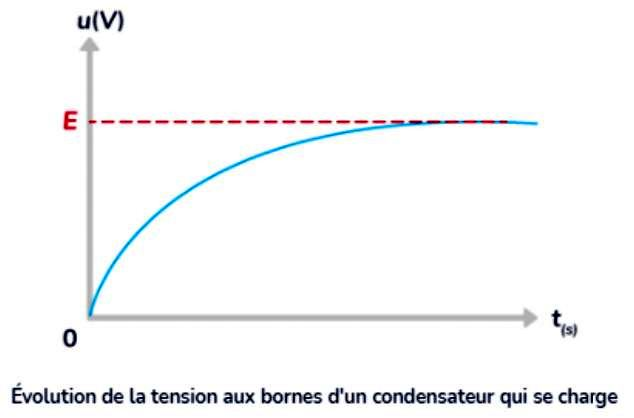
\includegraphics[width=0.7\linewidth]{imgs/p7/courbeCharge.jpg}
\end{figure}

La charge $q(t)$ évolue de la même manière (même fonction), avec la seule différence étant la valeur de l'asymptote qui correspond bien à $CE$. 

\begin{exo}
Comment évolue l'intensité du courant $i(t)$? Montrer grâce à un calcul. Montrez le graphique de $i(t)$. 
\vspace{5cm}
\end{exo}




\subsection{Circuit de décharge}

Comme nous avons vu dans la partie précédente, un condensateur se trouve soit dans un des deux états : 
\begin{itemize}
    \item Tant que le condensateur est branché sur un générateur, la tension $u_c $ et le condensateur accumule de la charge : il est en phase de charge. En mode charge, le condensteur est un récepteur. 
    \item En absence de la tension imposée par un générateur, la charge accumulée par le condensteur commence à dissiper et repartant dans le circuit, et la tension $u_c$ commence à diminuer : c'est la phase de décharge. En mode décharge le condensateur se comporte comme un \textbf{générateur}. 
\end{itemize}

\begin{figure}[H]
\centering
\begin{subfigure}{.55\textwidth}
  \centering
  % include first image
  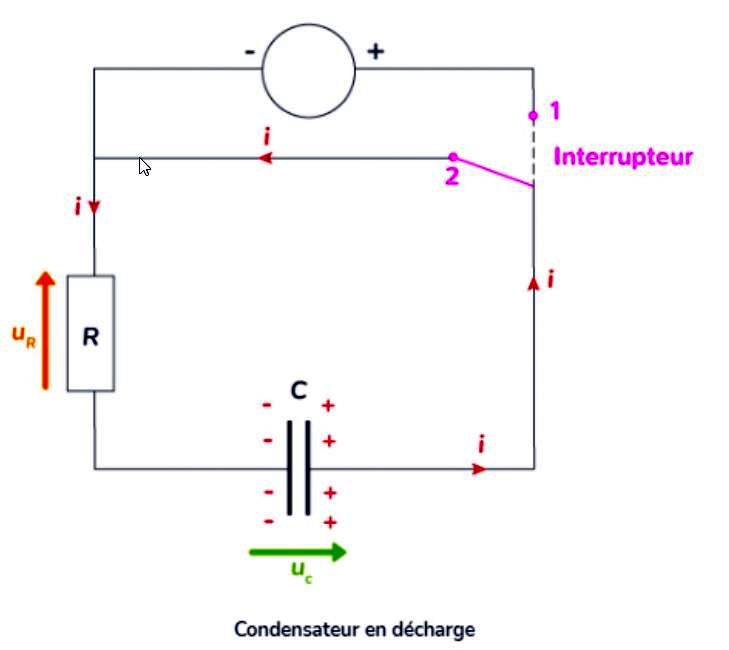
\includegraphics[width=.95\linewidth]{imgs/p7/RCdecharge.jpg}  
\end{subfigure}
\begin{subfigure}{.4\textwidth}
  \centering
  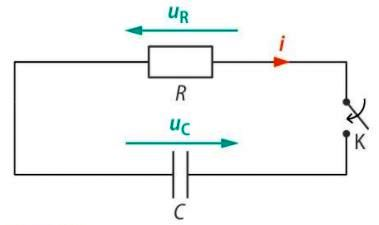
\includegraphics[width=.95\linewidth]{imgs/p7/rcDecharg2.jpg}  
\end{subfigure}
\caption{Décharge d'un condensateur dans une résistance.}
\end{figure}

En appliquant la même méthodologie que dans la partie précédente nous trouvons les équations suivantes pour $u_C(t)$ et $q(t)$: 
\begin{align}
    \od{u_C}{t} + \frac{1}{\tau}u_C &= 0 \\
    \od{q}{t} + \frac{1}{\tau}q &= 0
\end{align}
et leurs solutions : 
\begin{align}
    u_C(t) &= E\cdot e^{-\nicefrac{t}{\tau}} \\
    q(t) &= CE\cdot e^{-\nicefrac{t}{\tau}}
\end{align}

Voici comment la tension $u_C(t)$ évolue avec le temps : 

\begin{figure}[H]
    \centering
    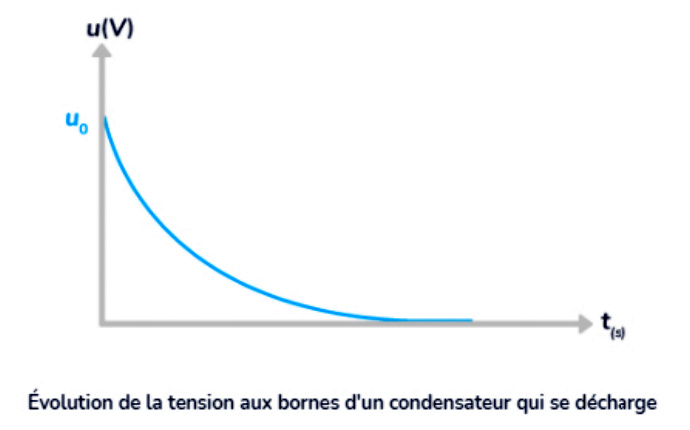
\includegraphics[width=0.7\linewidth]{imgs/p7/courbeDecharge.png.jpg}
\end{figure}

\begin{exo}
Faire la démonstration pour obtenir les équations (10) et (11), avec $\tau = RC$. Montrer comment nous obtenons les solutions (12) et (13). 
\vspace{10cm}
\end{exo}

\subsection{Détermination du $\tau$}

Il existe différentes manières de déterminer la valeur de la constante du temps $\tau$ graphiquement. Voici en quelques unes : 
\begin{itemize}
    \item Quand $t=\tau$ alors $u_c(\tau) = E\left(1-e^{-1}\right) = 0,63E$. En repérant l'abscisse correspondant à l'ordonnée $0,63E$, et cela correspondrait à $\tau$. 
    \item Dans le cas d'une courbe de décharge, $u_c(\tau) = E\cdot e^{-1} = 0,37E$.
    \item Une autre propriété de la fonction exponentielle est que la tangente à l'origine de la courbe ($u_C(t)$) coupe l'asymptote à l'abscisse $t=\tau$. Pour rappelle l'asympotote pour un condensateur en charge correspond à $u_C = E$, et pour un condensateur en décharge $u_C = 0$
\end{itemize}

\begin{figure}[H]
\centering
\begin{subfigure}{.49\textwidth}
  \centering
  % include first image
  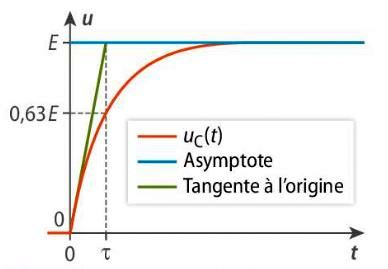
\includegraphics[width=.95\linewidth]{imgs/p7/courbeRC.jpg}  
\end{subfigure}
\begin{subfigure}{.43\textwidth}
  \centering
  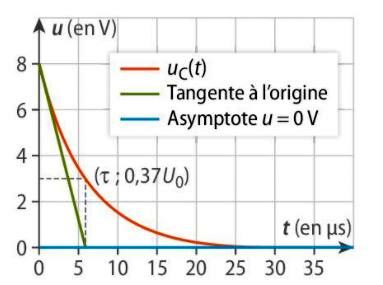
\includegraphics[width=.95\linewidth]{imgs/p7/courbeDecharge2.jpg}  
\end{subfigure}
\end{figure}

\begin{rmrq}
Une autre propriété de la fonction exponentielle (que nous avons déjà vu dans les autres chapitres où la fonction exponentielle est exploitée) est que au bout de $t\approx5\tau$ nous sommes passé en régime permanent. 
\end{rmrq}

\begin{exo}
Montrer que $t\approx5\tau$ est une bonne approximation de la durée du régime transitoire. 
\vspace{3cm}
\end{exo} 

\subsection{Influence des caractéristiques du circuit} 

Les deux facteurs qui influence la constante du temps, et par conséquent la durée de charge ou décharge sont - pas très étonnement - les valeurs de la résistance $R$ et de la capacité $C$. En variants ces valeurs nous pouvons changer la vitesse de charge/décharge du circuit (c.f. figure \ref{fig:tempsresist}). 

\begin{figure}[H]
\centering
\begin{subfigure}{.49\textwidth}
  \centering
  % include first image
  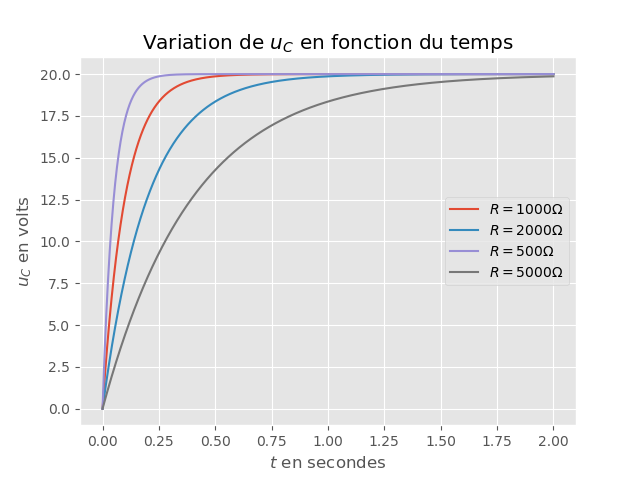
\includegraphics[width=\linewidth]{imgs/p7/Figure_1.png}  
\end{subfigure}
\begin{subfigure}{.49\textwidth}
  \centering
  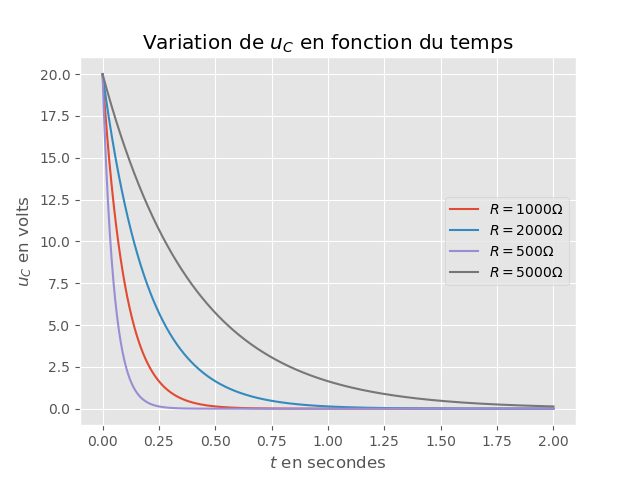
\includegraphics[width=\linewidth]{imgs/p7/Figure_2.png}  
\end{subfigure}
\caption{L'influence de la variation de la résistance sur la durée de charge (gauche) et de la décharge (droite).}
\label{fig:tempsresist}
\end{figure}








\end{document}